%\section{Traditional IP Networks}
\section{State of Quo in Networking}
\label{traditional_nets}

Computer networks can be divided in three planes of functionality: the
data, control and management planes (see Figure~\ref{fig:currentnetplanes}).  
The data plane corresponds to the networking devices, which are responsible 
for (efficiently) forwarding data.  The control plane represents the protocols 
used to populate the forwarding tables of the data plane elements. The management 
plane includes the software services, such as SNMP-based tools~\cite{presuhn2002}, 
used to remotely monitor and configure the control functionality.  Network policy 
is defined in the management plane, the control plane enforces the policy, and the 
data plane executes it by forwarding data accordingly.

\begin{figure}[t!]
\centering
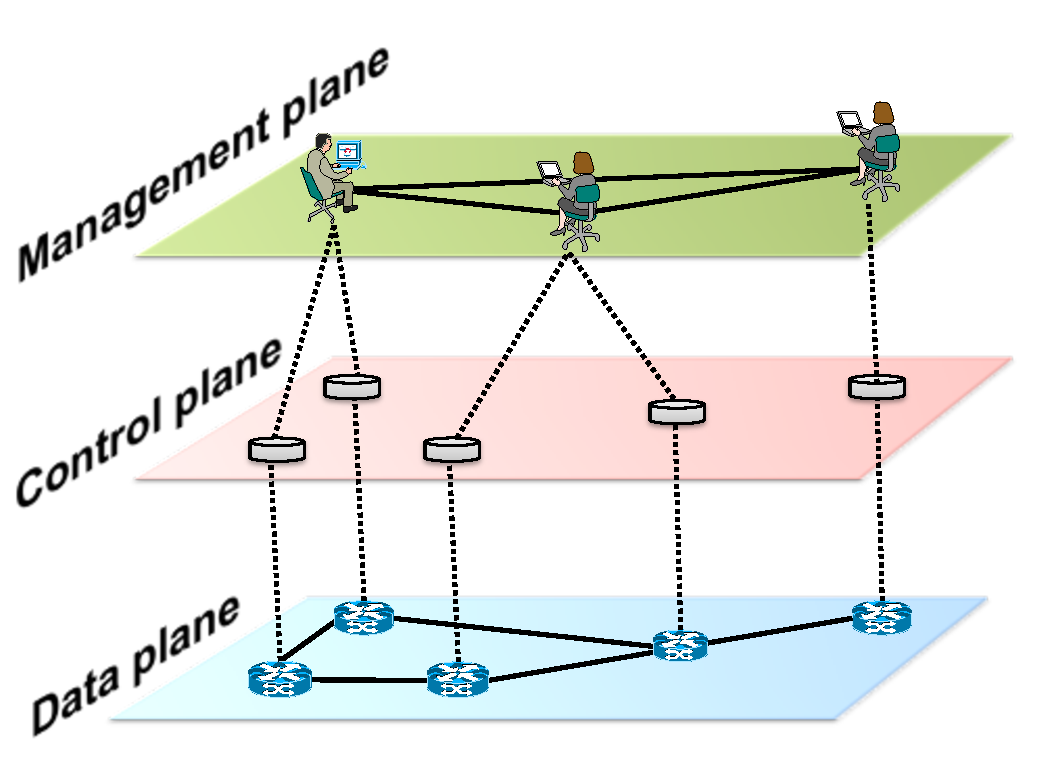
\includegraphics[width=0.75\columnwidth]{figures/fig2_network_functionality.pdf}
\caption{Layered view of networking functionality.}
\label{fig:currentnetplanes}
\end{figure}

In traditional IP networks, the control and data planes are tightly coupled, and 
embedded in the same networking devices, and the whole structure is highly decentralized.
This was considered important for the design of the Internet in the early days: it seemed 
the best way to guarantee network resilience, which was a crucial design goal. In fact, 
this approach has been quite effective in terms of network performance, with a rapid 
increase of line rate and port densities.

However, the outcome is a very complex and relatively static architecture. It is also the 
fundamental reason why traditional networks are rigid, and complex to manage and control.
These two characteristics are largely responsible for a vertically-integrated industry where 
innovation is difficult.

Network misconfigurations and related errors are extremely common in today's networks. 
For instance, more than 1000 configuration errors have been observed in BGP 
routers~\cite{feamster2005}. A single misconfigured device can be a big 
headache for network operators and may have extremely severe consequences. Indeed, while
rare, a single misconfigured router is able to compromise the correct operation of the 
whole Internet for hours~\cite{barrett1997,butler2010}. 

To support network management, a small number of vendors offer proprietary solutions of 
specialized hardware, operating systems, and control programs (network applications). 
Network operators have to acquire and maintain different management solutions and the 
corresponding specialized teams.  The capital and operational cost of building and 
maintaining a networking infrastructure is significant, with long return on investment 
cycles, which hamper innovation and addition of new features and services (for instance 
access control, load balancing, energy efficiency, traffic engineering).  
To alleviate the lack of in-path functionalities within the network, a myriad of specialized 
components and middleboxes, such as firewalls, intrusion detection systems and deep packet inspection engines, proliferate 
in current networks. A recent survey of 57 enterprise networks shows that the number of 
middleboxes is already on par with the number of routers in current networks~\cite{sherry2012}.
Despite helping in-path functionalities, the net effect of middleboxes has been increased
complexity of network design and its operation.

% EOF: 1_traditionl_nets.tex
